\section{Руководство пользователя и примеры использования}
\subsection{Введение}


\subsection{Общая диаграмма комплекса}
% 	Math net  статья
    
    
\subsection{Надстройка}
%ПЕРЕХОД
Архитектура разработанной надстройки над существующей библиотекой локального логико-вероятностного вывода представлена на диаграмме классов Рис. \ref{Structure}.

\begin{figure}[h!]
\begin{center}
\includegraphics[width=\linewidth]{Structure.png}
\caption{Диаграмма классов расширения библиотеки локального вывода.}
\label{Structure}
\end{center}
\end{figure}

Абстрактный класс BaseKnowledgePattern определяет ту функциональность, которую должны иметь наследующие от него классы: Scalar\-KnowledgePattern и IntervalKnowledgePattern.

Класс ScalarKnowledgePattern реализует расширение фрагмента знаний со скалярными (точечными) оценками вероятности истинности элементов. Он содержит два вида конструктора: одному на вход передается глобальный индекс, другому -- глобальный индекс и массив с оценками вероятности истинности. Имеется отдельный метод для задания оценок элементов ФЗ. Помимо этого, реализованы методы, которые осуществляют поддержание локальной непротиворечивости, решают задачи априорного и апостериорного локального логико-вероятностного вывода. Реализованные методы полностью покрывают требуемую функциональность.

Класс IntervalKnowledgePattern реализует расширение фрагмента знаний с интервальными оценками вероятности истинности элементов. Его методы имеют аналогичную, ранее рассмотренному классу Scalar\-KnowledgePattern, функциональность.


\subsection{Внедрение парсера}

Объемлющий проект AlgBN Web App~\ref{App} по работе с алгебраическими байесовскими сетями включает в себя математическую библиотеку AlgBN Math Library по работе с локальными структурами АБС и осуществлению локального логико-вероятностного вывода над ними.  

\begin{figure}[h!]
\begin{center}
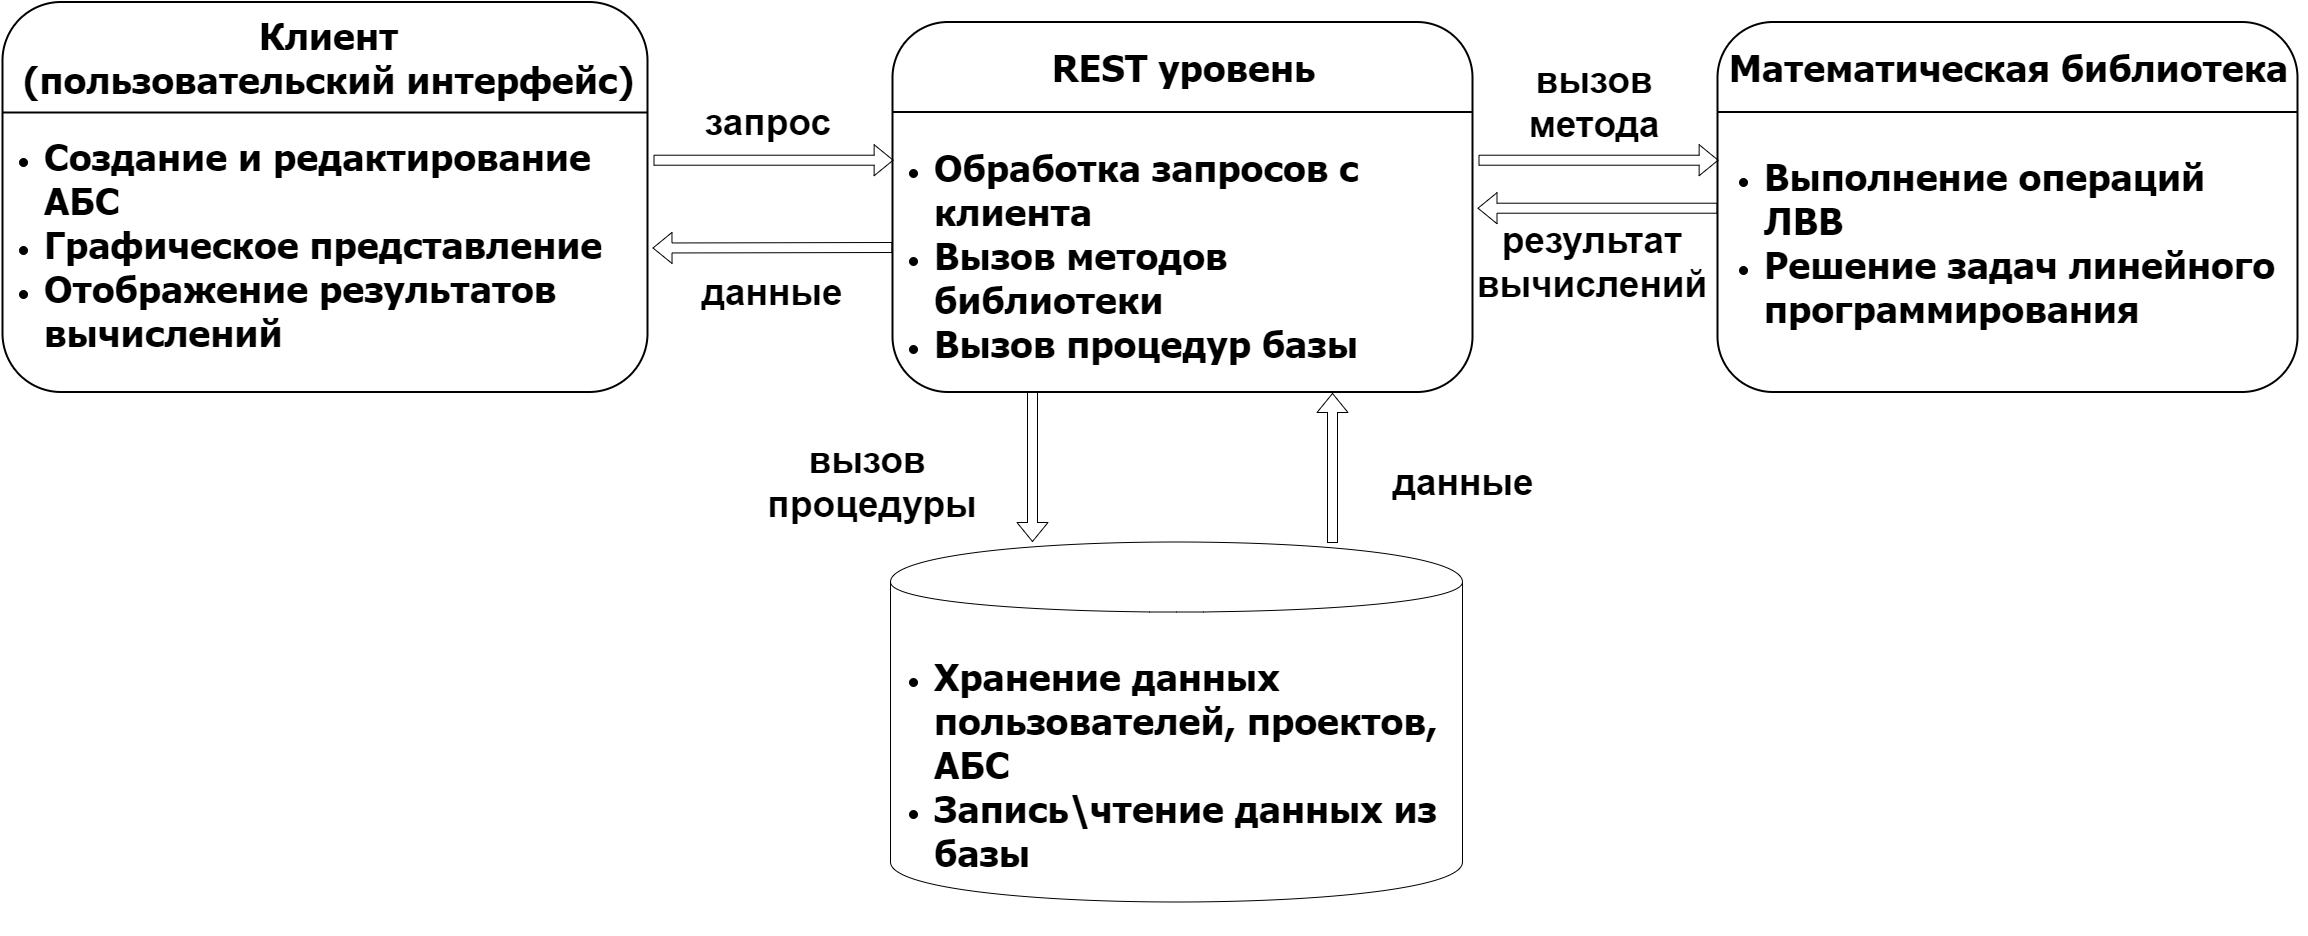
\includegraphics[width=.9\textwidth]{App}
\caption{Диаграмма проекта AlgBN Web App}
\label{App}
\end{center}
\end{figure}

Структура Inferer~\ref{Inf} в библиотеке осуществляет не только проверку и поддержание непротиворечивости во фрагменте знаний, но и решение задачи априорного вывода для пропозициональных формул, заданных над тем же алфавитом, что и обрабатываемый ФЗ. 

\begin{figure}[h!]
\begin{center}
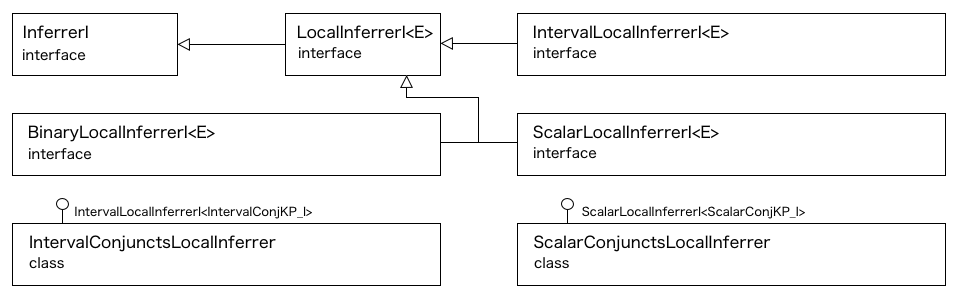
\includegraphics[width=\textwidth]{Inferrers}
\caption{Диаграмма структуры Inferer}
\label{Inf}
\end{center}
\end{figure}

В AlgBN Math Library для упрощения работы с АБС был внедрен парсер~\cite{nsmv_apr} пропозициональных формул. Если раньше приходилось строить характеристический вектор для поступающей формулы вручную, то на данном этапе в метод поступает формула в виде строки, а далее ее обрабатывает парсер, строя для нее характеристический вектор. Такая автоматизация позволяет избежать ошибок при построении характеристического вектора.

\subsubsection{Пример решения задачи априорного вывода для скалярных ФЗ}

Приведем пример вызова метода для осуществления априорного вывода в библиотеки для фрагмента знаний со скалярными оценками вероятности истинности и пропозициональной формулы $f_1 = x_0 \rightarrow x_1$:

\begin{lstlisting}[label=list1,caption={Пример решения задачи априорного вывода для скалярного ФЗ},escapeinside={(*}{*)}]
public void aprioriInferenceTest(){= 0.6;
ArrayAlphabet alphabet = new ArrayAlphabet(new string[] { "x0", "x1", "x2" });
double[] bound = { 1, 0.7, 0.5, 0.3 };
ScalarKnowledgePattern scKP = new ScalarKnowledgePattern(alphabet, Convert.ToInt64("11", 2), new double[][] { bound });
double result = scKP.aprioriInference("x0=>x1", 2);
}
\end{lstlisting}

Для рассматриваемой формулы парсер построит следующий характеристический вектор: $\chi_{f_1} = \left( \begin{array}{c}
1\\
1\\
0 \\
1
\end{array}  \right)$. Далее для него будет посчитан вектор ${\bf L}_{f_1} = \left( \begin{array}{c}
1\\
0\\
-1 \\
1
\end{array}  \right)$, который в последствии будет использован в уравнении априорного вывода. Результатом выполнения системы операторов будет вероятность формулы $p(f_1) = 0.6$.



Пример для фрагмента знаний со скалярными оценками вероятности истинности и пропозициональной формулы $f_2 = x_0 \vee x_1$:

\begin{lstlisting}[label=list1,caption={Пример решения задачи априорного вывода для скалярного ФЗ},escapeinside={(*}{*)}]
public void aprioriInferenceTest1()
{
double expectedResultLB = 0.9;
ArrayAlphabet alphabet = new ArrayAlphabet(new string[] { "x0", "x1", "x2" });
double[] bound = { 1, 0.8, 0.7, 0.6 };
ScalarKnowledgePattern scKP = new ScalarKnowledgePattern(alphabet, Convert.ToInt64("11", 2), new double[][] { bound });
double result = scKP.aprioriInference("x1|x0", 2)[0];    
Assert.AreEqual(expectedResultLB, result, 0.0001);

}
\end{lstlisting}

Для рассматриваемой формулы парсер построит следующий характеристический вектор: $\chi_{f_2} = \left( \begin{array}{c}
0\\
1\\
1 \\
1
\end{array}  \right)$. Далее для него будет посчитан вектор ${\bf L}_{f_2} = \left( \begin{array}{c}
0\\
1\\
1 \\
-1
\end{array}  \right)$, который в последствии будет использован в уравнении априорного вывода. Результатом выполнения системы операторов будет вероятность формулы $p(f_2) = 0.9$.


\subsubsection{Пример решения задачи априорного вывода для интервального ФЗ}
Пример для ФЗ с интервальными оценками вероятности истинности и пропозициональной формулы $f_3 = x_1 \leftrightarrow x_1$:

\begin{lstlisting}[label=list1,caption={Пример решения задачи априорного вывода для интервального ФЗ},escapeinside={(*}{*)}]
public void aprioriInferenceTest(){
double expectedResultLB = 0.46, expectedResultUB = 1;
ArrayAlphabet alphabet = new ArrayAlphabet(new string[] { "x0", "x1", "x2" });
double[] Lbound = { 1, 0.46, 0.29, 0.33 };
double[] Ubound = { 1, 0.7, 0.5, 0.9 };
IntervalKnowledgePattern intKP = new IntervalKnowledgePattern(alphabet, Convert.ToInt64("11", 2), new double[][] { Lbound, Ubound });
double[] result = intKP.aprioriInference("x0<=>x1", 2); 
}
\end{lstlisting}


Для рассматриваемой формулы парсер построит следующий характеристический вектор: $\chi_{f_3} = \left( \begin{array}{c}
1\\
0\\
0 \\
1
\end{array}  \right)$. Далее для него будет посчитан вектор ${\bf L}_{f_3} = \left( \begin{array}{c}
1\\
-1\\
-1 \\
2
\end{array}  \right)$, который в последствии будет использован в уравнении априорного вывода. В данном случае будет построена ЗЛП. Результатом выполнения системы операторов будет вероятность формулы $p(f_3) = [0.46, 1]$.




\subsection{Чувствительность}
%ПЕРЕХОД
Основным случаем анализа чувствительности локального апостериорного вывода в алгебраических байесовских сетях является анализ поведения оценки чувствительности $\epsilon$ первой задачи апостериорного вывода для фрагмента знаний~(ФЗ), построенного над идеалом конъюнктов, со скалярными оценками вероятности истинности и детерминированного свидетельства. Рассматривается допустимая вариация $\delta$ оценок фрагмента знаний в условиях фиксации исходного набора оценок ($\mathbf{P_{c}} = \mathbf{P_{c_0}}$).

Зададим ФЗ $(C, \mathbf{P_{c_0}})$ над алфавитом из двух атомов $A = \{ a_1, a_0 \}$. Следующий вектор состоит из скалярных оценок ФЗ:
\begin{equation*}
\Pc^{\circ} = \begin{pmatrix} 1 \\ p(x_1) \\ p(x_2) \\p(x_2x_1) \end{pmatrix} = \begin{pmatrix} 1 \\ 0.6 \\ 0.5 \\0.333 \end{pmatrix}. 
\end{equation*}

Для заданного ФЗ будем решать первую задачу апостериорного вывода со следующими детерминированными свидетельствами:
\begin{equation*}
\langle x_{1}\rangle;\langle ,x_{1}\rangle; \langle x_{2}\rangle;\langle x_{2}, x_{1} \rangle;  \langle x_{1}, x_{2} \rangle.
\end{equation*}

Перечисленные выше свидетельства соответствуют соответственно следующим пропозициональным формулам:
\begin{equation*}
x_{1}; \overline{x_{1}}; x_{2}; x_{2}\overline{x_{1}}; \overline{x_{2}}x_{1}.
\end{equation*}

Данным свидетельствам соответствуют следующие вектора-редистрибъютеры:
\begin{equation*}
\mathbf{r}^{\langle x_{1} \rangle} = \begin{pmatrix} 0 \\ 0 \\ 1 \\ 0 \end{pmatrix}; 
\mathbf{r}^{\langle x_{1} \rangle} = \begin{pmatrix} 1 \\ 0 \\ -1 \\ 0 \end{pmatrix};
\mathbf{r}^{\langle x_{2} \rangle} = \begin{pmatrix} 0 \\ 1 \\ 0 \\ 0 \end{pmatrix}; 
\end{equation*}
\begin{equation*}
\mathbf{r}^{\langle x_{2}, x_{1} \rangle} = \begin{pmatrix} 0 \\ 0 \\ 1 \\ -1 \end{pmatrix};
\mathbf{r}^{\langle x_{1}, x_{2} \rangle} = \begin{pmatrix} 0 \\ 1 \\ 0 \\ -1 \end{pmatrix}.
\end{equation*}
Для каждого свидетельства и и фиксированного $\delta$ (выбранной вариации вектора оценок вероятности истинности) вычислим оценку чувствительности $\epsilon$. Решим задачу линейного программирования~(ЗЛП) по поиску минимума и максимума следующего выражения:
\begin{equation*}
\p\evidence - \widehat{p}\evidence
\end{equation*}

\noindent при ограничениях:
\begin{equation}\label{eq:boundary1} \In \Pc\geq 0,\end{equation}
\begin{equation}\label{eq:boundary2} \Pc = \Pc^{\circ},    \end{equation}
\begin{equation}\label{eq:boundary3}\In \PcHat \geq 0,    \end{equation}
\begin{equation}\label{eq:boundary4} v(\Pc, \PcHat) \leq \delta,    \end{equation}
\begin{equation}\label{eq:boundary5}\p\evidence=(\redistributor,\Pc),     \end{equation}
\begin{equation}\label{eq:boundary6}\widehat{p}\evidence=(\redistributor,\PcHat),    \end{equation}
\begin{equation}\label{eq:boundary7} \PcHat[i] = 1.\end{equation}

В первом блоке~(\ref{eq:boundary1}) ограничений задаются условия на непротиворечивость оценок вероятности истинности элементов рассматриваемого вектора $\Pc$. 
С помощью второго блока~(\ref{eq:boundary2}) фиксируются скалярные оценки исходного вектора. 
В третьем блоке~(\ref{eq:boundary3}) задаются условия на непротиворечивость варьируемого вектора $\PcHat$. Четвертый~(\ref{eq:boundary4}) -- накладывает ограничения на вариативность. 
Следующие два ограничения~(\ref{eq:boundary5}, \ref{eq:boundary6}) задают то, каким образом решения первой задачи апостериорного вывода для фиксированного свидетельства и векторов $\Pc$ и $\PcHat$ выражаются через элементы этих векторов соответственно. Последнее условие~(\ref{eq:boundary7}) гарантирует нам выполнение необходимого условия того, что вероятность пустой конъюнкции в варьируемом векторе будет равна 1.

\begin{table}[htbp]
\caption{Оценки чувствительности для детерминированных свидетельств.} 
\begin{center}
\begin{tabular}{ |c|c|c|c|c|c|c|c|c| }
\hline
Свид-во &     $\delta= .01$ & $ .07$ & $ .15$ & $.27$ & $.43$ & $.58$ & $.7$ & $1$ \\ \hline
$\langle x_{2}, x_{1} \rangle$ & $.02$ & $.14$ & $.3$ & $.503$ & $.663$ & $.813$ & $.833$ & $.833$ \\
$\langle x_{2} \rangle$ & $.01$ & $.07$ & $.15$ & $.27$ & $.4$ & $.4$ & $.4$ & $.4$ \\
$\langle x_{1}, x_{2} \rangle$ & $.02$ & $.14$ & $.3$ & $.503$ & $.663$ & $.733$ & $.733$ & $.733$ \\
$\langle x_{1} \rangle$ & $.01$ & $.07$ & $.15$ & $.27$ & $.43$ & $.5$ & $.5$ & $.5$ \\
$\langle , x_{1} \rangle$ & $.01$ & $.07$ & $.15$ & $.27$ & $.43$ & $.5$ & $.5$ & $.5$ \\\hline
\end{tabular}
\end{center}
\label{tabular:sense}
\end{table}

В таблице \ref{tabular:sense} приведены оценки чувствительности для фиксированных дельт и набора рассматриваемых детерминированных свидетельств. На некоторых интервалах значений дельты прослеживается линейная зависимость дельты и получаемой оценки чувствительности. 

\begin{figure}[htbp]
\centerline{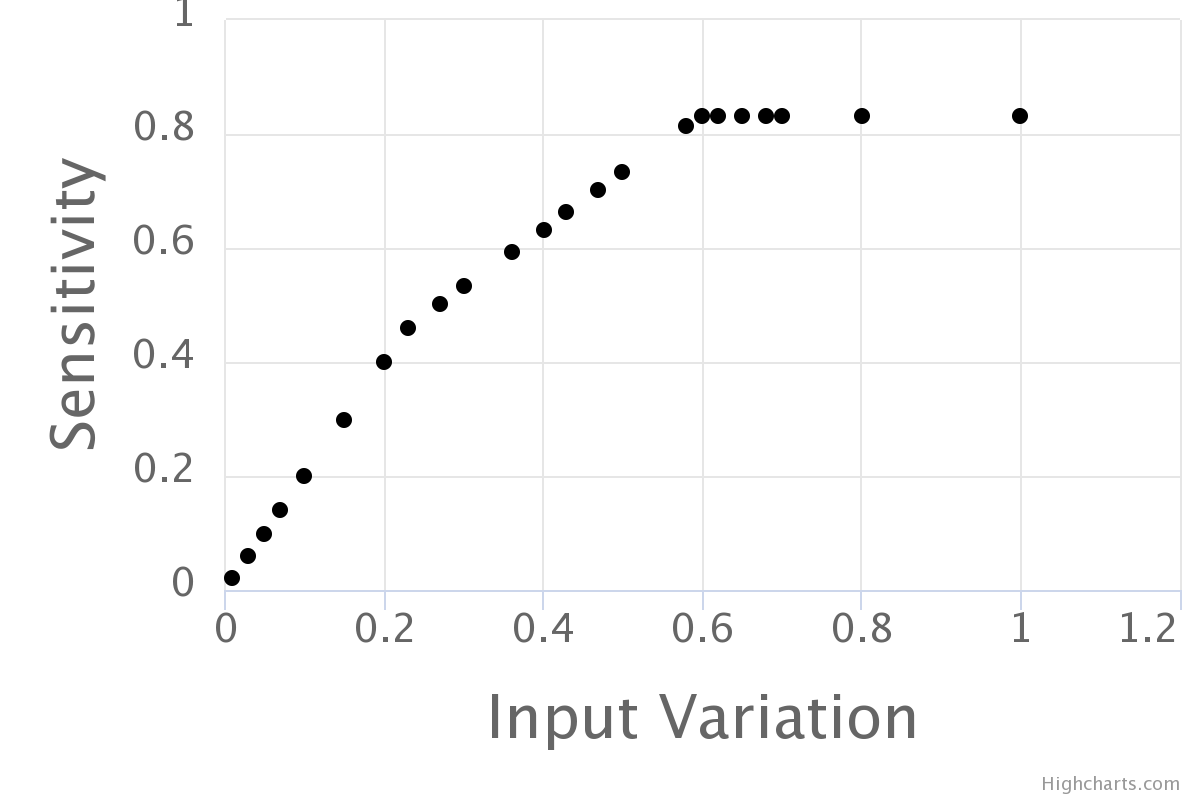
\includegraphics[width=0.8\textwidth]{chart_1.png}}
\caption{График оценок чувствительности для детерминированного свидетельства  $\langle x_{2}, x_{1} \rangle$}
\label{chart1}
\end{figure}

На рис.\ref{chart1} представлен график роста оценки чувствительности с ростом допустимой вариации исходного вектора в рамках рассматриваемой первой задачи апостериорного вывода для детерминированного свидетельства $\langle x_{2}, x_{1} \rangle$ и кванта $x_{2} \overline{x_{1}}$, в виде которого она может быть представлена.

\begin{figure}[htbp]
\centerline{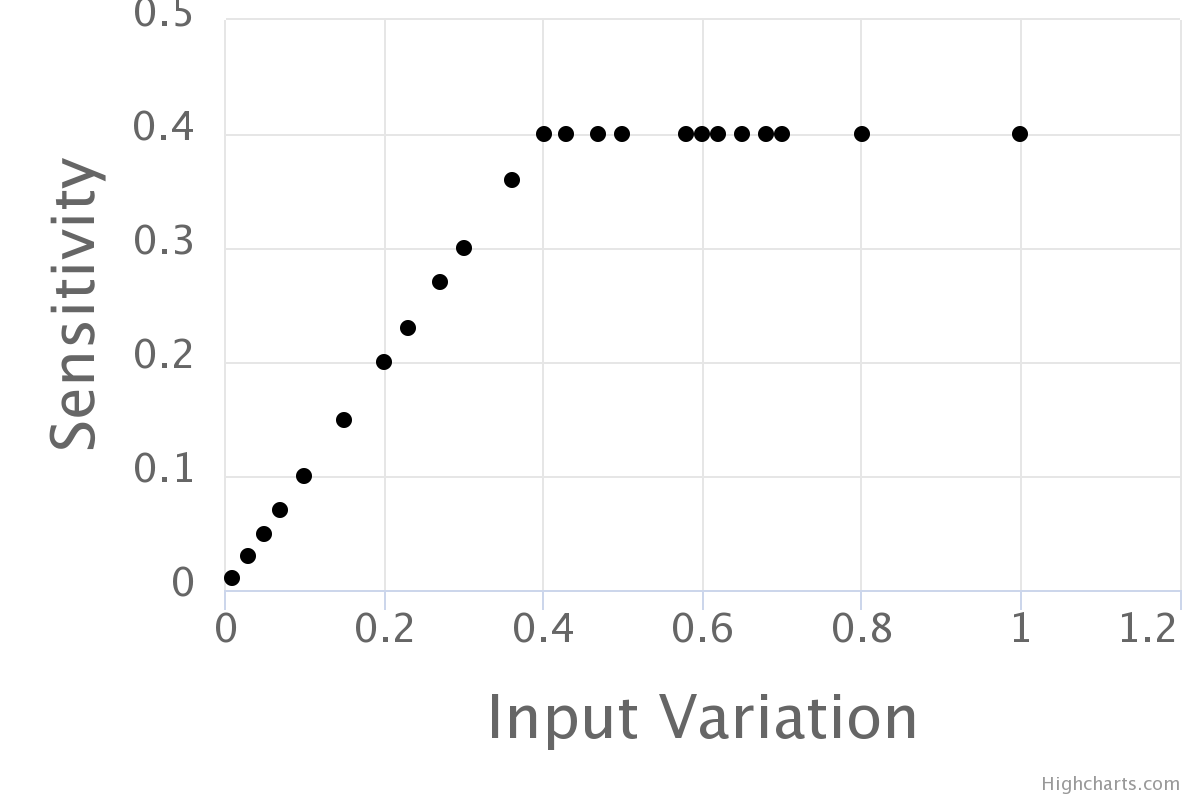
\includegraphics[width=0.8\textwidth]{chart_2.png}}
\caption{График оценок чувствительности для детерминированного свидетельства  $\langle x_{2} \rangle$}
\label{chart2}
\end{figure}

На рис.\ref{chart2} представлен график роста оценки чувствительности с ростом допустимой вариации исходного вектора в рамках рассматриваемой первой задачи апостериорного вывода для детерминированного свидетельства $\langle x_{2}\rangle$ и кванта $x_{2}$, в виде которого она может быть представлена.

\begin{figure}[htbp]
\centerline{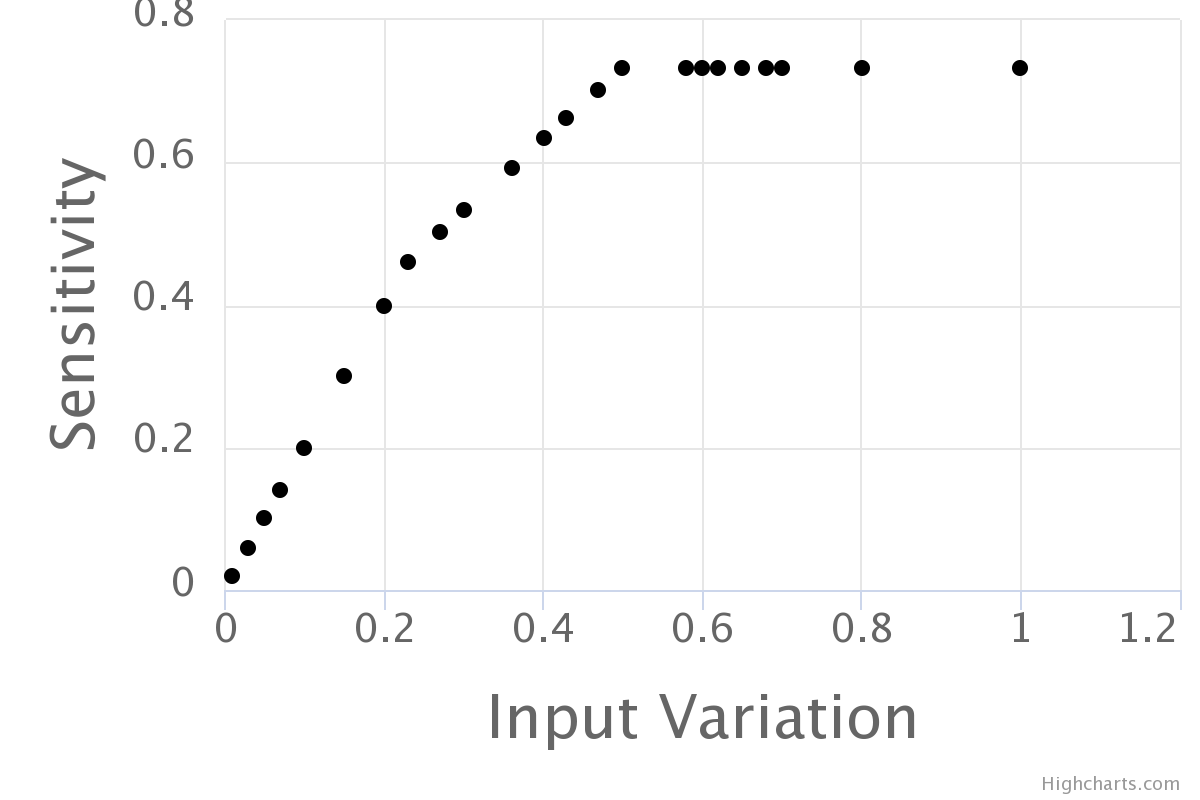
\includegraphics[width=0.8\textwidth]{chart_3.png}}
\caption{График оценок чувствительности для детерминированного свидетельства  $\langle x_{1}, x_{2} \rangle$}
\label{chart3}
\end{figure}

На рис.\ref{chart3} представлен график роста оценки чувствительности с ростом допустимой вариации исходного вектора в рамках рассматриваемой первой задачи апостериорного вывода для детерминированного свидетельства $\langle x_{1}, x_{2} \rangle$ и кванта $\overline{x_{2}} x_{1}$, в виде которого она может быть представлена.

\begin{figure}[htbp]
\centerline{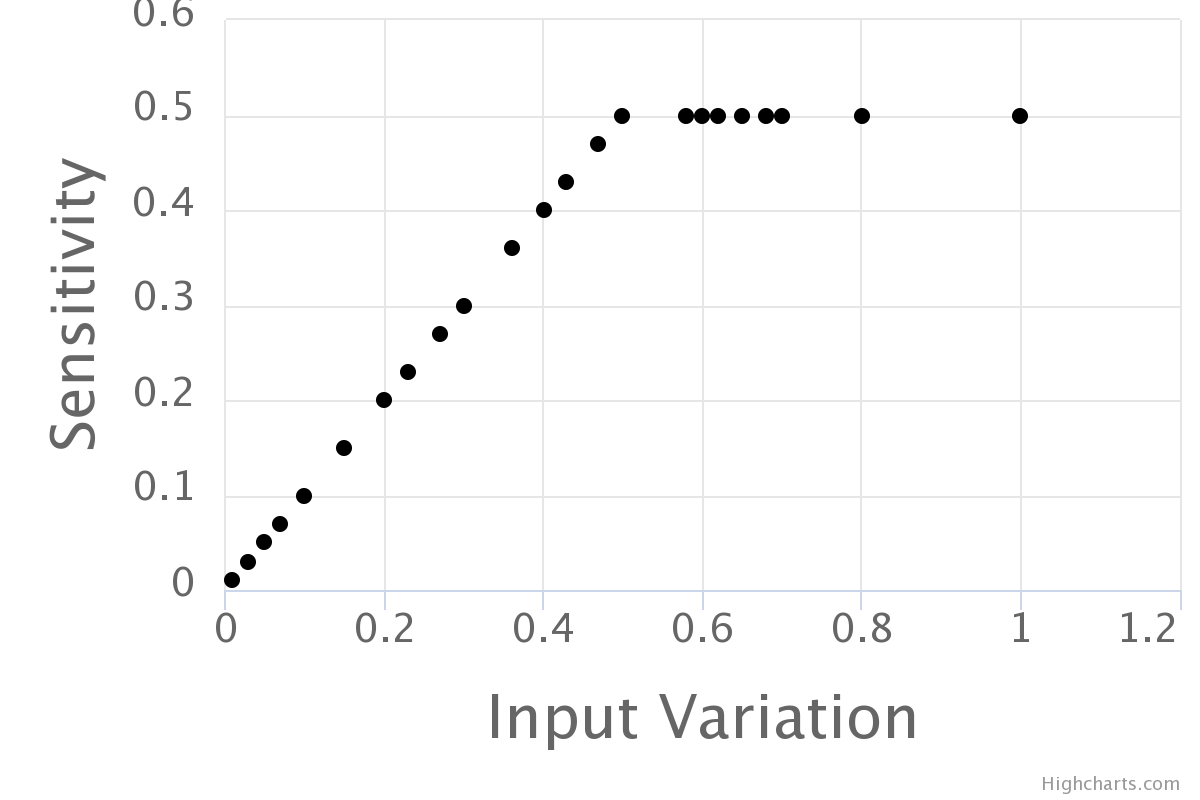
\includegraphics[width=0.8\textwidth]{chart_4.png}}
\caption{График оценок чувствительности для детерминированных свидетельств  $\langle  x_{1} \rangle$ и $\langle , x_{1} \rangle$}
\label{chart4}
\end{figure}

На рис.\ref{chart4} представлен график роста оценки чувствительности с ростом допустимой вариации исходного вектора в рамках рассматриваемой первой задачи апостериорного вывода для детерминированных свидетельств $\langle x_{1} \rangle$ и $\langle , x_{1} \rangle$, с квантами $x_{1}$ и $\overline{x_{1}}$ соответственно. Для обоих случаев график зависимости, как было показано экспериментально, совпал.

Как можно видеть из приведенных графиков, зависимость оценки чувствительности результата решения задачи первого вывода для представленных свидетельств выражается линейно на некоторых интервалах. Показано, что чувствительность возрастает при возрастании дельта, а потом стабилизируется.

    
\subsection{Выводы по главе}